%\documentclass[12pt, handout]{beamer}
\documentclass[12pt]{beamer}

\usepackage{cmap}
\usetheme{Madrid}
\usepackage[utf8]{inputenc}
\usepackage[russian]{babel}
\usepackage[OT1]{fontenc}
\usepackage{amsmath}
\usepackage{amsfonts}
\usepackage{amssymb}
\usepackage{graphicx}
\usepackage{listings}

\author{Игорь Рязанцев}
\title{Файлы и ввод-вывод в Python}
\institute{Лекция 03}
\date{2021г.}

%\setbeamercovered{transparent} 
\setbeamertemplate{navigation symbols}{} 
%\logo{} 
%\institute{} 
%\date{} 
%\subject{} 

\begin{document}

\begin{frame}
\titlepage
\end{frame}

\begin{frame}{Тестовое задание [Лекция 02]}
\textbf{\# Необходимо описать класс осветительной установки, создать список объектов и вывести на экран спецификацию объекта освещения.} \\
\center{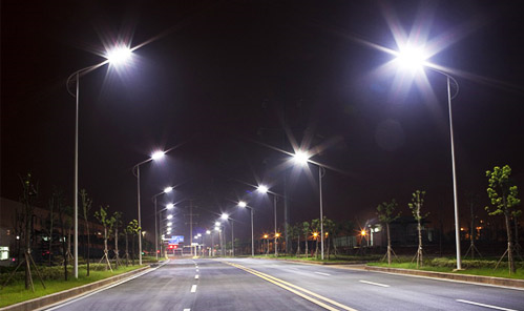
\includegraphics[scale=0.6]{image/road.png}}
\end{frame}

\begin{frame}[t]{Оглавление}
\tableofcontents[part=1]
\end{frame}

%\begin{frame}[t]{Оглавление}
%\tableofcontents
%\end{frame}


\part{1}
\section{Понятие файла}
\begin{frame}{Понятие файла}
\textbf{Файл} -- это помеченная (именованная) область на каком-либо носителе. \\
\vspace{0.5cm}

\begin{tabular}{|p{0.3cm}|p{0.3cm}|p{0.3cm}|p{0.3cm}|p{0.3cm}|p{0.3cm}|p{0.3cm}|p{0.3cm}|p{0.55cm}|p{0.55cm}|p{0.3cm}|p{0.3cm}|p{0.3cm}|p{0.3cm}|p{0.3cm}|p{0.3cm}|}
\hline 
\multicolumn{8}{|c|}{Байт} & Бит & Бит &  &  &  &  &  &  \\ 
\hline 
0 & 0 & 1 & 0 & 0 & 0 & 0 & 0 & 0 & 0 & 0 & 1 & 0 & 1 & 1 & 1 \\ 
\hline 
\multicolumn{16}{c}{} \\ 
\multicolumn{16}{|c|}{file.txt} \\ 
\hline 
\end{tabular} 
\par
\vspace{0.3cm}
\begin{tabular}{|c|c|}
\hline 
Код\footnote{Кодировка ASCII} & Символ \\ 
\hline 
32 & Пробел \\ 
\hline 
33 & ! \\ 
\hline 
\end{tabular}  
\par 
\vspace{0.3cm}
$0\times2^7$ + $0\times2^6$ + $1\times2^5$ + $0\times2^4$ + $0\times2^3$ + $0\times2^2$ + $0\times2^1$ + $0\times2^0$ = 32 \\
\end{frame}


\section{Типы файлов}
\begin{frame}{Типы файлов}
\textbf{Типы фалов:}
\begin{itemize}
\item Текстовые файлы:
	\begin{itemize}
		\item 1 Байт = символ;
		\item Просмотреть файл можно с помощью текстового редактора;
		\item Текст разбит на строки (символ перевода строки)
	\end{itemize}
\item Бинарные файлы (двоичные файлы):
	\begin{itemize}
		\item 1 Байт = тоже символ, но смысл несет комбинация байтов, которая определена структурой сохраненной информации;
		\item Просмотреть файл тоже можно с помощью текстового редактора, но без понимания структуры ее смысл не будет ясен (как незнакомый язык, звуки слышишь, но не понимаешь о чем говорят); 
	\end{itemize}
\end{itemize}
\end{frame}


\section{Текстовые файлы}
\subsection{Чтение из файла}
\begin{frame}{Текстовые файлы}
\textbf{\# Чтение файла} \\
\vspace{0.5cm}
\lstinputlisting[language=Python]{code/33.py}
\vspace{0.5cm}
Результат: \\
\lstinputlisting[language=Python]{code/33_1.py}
\end{frame}


\begin{frame}{Текстовые файлы}
\textbf{\# Чтение файла} \\
\vspace{0.5cm}
\lstinputlisting[language=Python]{code/34.py}
\vspace{0.5cm}
Результат: \\
line 1 \\
line 2 \\
line 3 \\
\end{frame}


\subsection{Запись в файл}
\begin{frame}{Текстовые файлы}
\textbf{\# Запись в новый файл} \\
\vspace{0.5cm}
\lstinputlisting[language=Python]{code/35.py}
\vspace{0.5cm}
Результат (в файле): \\
\lstinputlisting[language=Python]{code/new_file.txt}
\end{frame}

\begin{frame}{Текстовые файлы}
\textbf{\# Присоединение данных к файлу (режим <<a>>)} \\
\vspace{0.3cm}
\lstinputlisting[language=Python]{code/36.py}
\vspace{0.5cm}
Результат (в файле): \\
\lstinputlisting[language=Python]{code/new_file2.txt}
\end{frame}

\section{Бинарные (двоичные) файлы}
\begin{frame}{Бинарные (двоичные) файлы}
\textbf{\# Запись в текстовой файл} \\
\vspace{0.5cm}
\lstinputlisting[language=Python]{code/38_1.py}
\vspace{0.5cm}
Результат в файле (10 байт): \\
4294967295 \\
\end{frame}


\subsection{Запись в файл}
\begin{frame}{Бинарные (двоичные) файлы}
\textbf{\# Бинарные файлы в отличие от текстовых хранят информацию в виде набора байт} \\
\vspace{0.3cm}
\textbf{\# Запись в бинарный файл} \\
\vspace{0.5cm}
\lstinputlisting[language=Python]{code/38_2.py}
\vspace{0.5cm}
Результат в файле (4 байт): \\
яяяя \\
\end{frame}


\subsection{Чтение из файла}
\begin{frame}{Бинарные (двоичные) файлы}
\textbf{\# Чтение из бинарного файла} \\
\vspace{0.5cm}
\lstinputlisting[language=Python]{code/38_3.py}
\vspace{0.5cm}
Результат в файле (4 байт): \\
4294967295 \\
\end{frame}


\begin{frame}{Тестовое задание}
\textbf{\# Необходимо сохранить список светильников в текстовом файле} 
\vspace{0.5cm}
\lstinputlisting[language=Python]{code/17.py}
\vspace{0.5cm}
Результат (в файле): \\
LED1  40  6000 \\
LED2 60  9000 \\
LED3 90 12000 \\
LED4 80 12000 \\
\end{frame}


\section{Ввод-вывод данных}
\begin{frame}[t]{Оглавление}
\tableofcontents[currentsection]
\end{frame}


\subsection{Ввод данных с клавиатуры}
\begin{frame}{Ввод данных с клавиатуры}
Ввод данных с клавиатуры осуществляется с помощью функции \textbf{input()}. После выполнения  функции программа ожидает ввода данных и после нажатия <<Enter>> записывает их в переменную. \\
\vspace{0.3cm}
\textbf{\# Ожидает ввод целого числа} 
\lstinputlisting[language=Python]{code/39_1.py}
\vspace{0.3cm}
\textbf{\# Ожидает ввод вещественного числа} 
\lstinputlisting[language=Python]{code/39_2.py}
\vspace{0.3cm}
\textbf{\# Ожидает ввод сроки} 
\lstinputlisting[language=Python]{code/39_3.py}
\end{frame}

\begin{frame}{Ввод данных с клавиатуры}
\textbf{\# Пример:} 
\vspace{0.5cm}
\lstinputlisting[language=Python]{code/40.py}
\vspace{0.5cm}
Результат (в файле): \\
Please, type your name: Bob \\
Your name is Bob \\
\end{frame}


\begin{frame}{Тестовое задание}
Напишите программу, которая запрашивает у пользователя:
\begin{itemize}
\item Имя (например, "What is your name?")
\item Возраст ("How old are you?")
\item Место жительства ("Where are you live?")
\end{itemize}
\vspace{0.3cm}
\textbf{Вывести на экран:} \\
This is имя \\
It is возраст \\
(S)he live in место\_жительства \\ 
\end{frame}


\begin{frame}{Тестовое задание}
Напишите программу, которая запрашивает у пользователя список из 4 светильников с характеристиками мощности и светового потока): \\
\vspace{0.3cm}
\textbf{Вывести на экран данные введенные пользователем:} \\
LED1  40  6000 \\
LED2 60  9000 \\
LED3 90 12000 \\
LED4 80 12000 \\
\end{frame}


\begin{frame}{Что мы изучили}
\begin{itemize}
\item Переменные 
\item Кортежи
\item Списки (вставка, удаление, сортировка)
\item Циклы \textbf{for}
\item Оператор \textbf{if}
\item Функции
\item Классы (наследование)
\item Импорт модулей
\item Файлы
\item Ввод-вывод 
\end{itemize}
\end{frame}


\begin{frame}{Что мы не изучили}
\begin{itemize}
\item Исключения try...catch
\item Асинхронность
\end{itemize}
\end{frame}


\section{Запуск программы без IDE}
\begin{frame}{Запуск программы без IDE}
\textbf{\# Windows} 
\begin{itemize}
\item python.exe имя\_программы.py
\end{itemize}
\vspace{0.3cm}
\textbf{\# Linux} 
\begin{itemize}
\item python3 ./имя\_программы.py
\end{itemize}
\end{frame}

\section{Сборка программы (.exe)}
\begin{frame}{Сборка программы (.exe)}
\textbf{\# PyInstaller} 
\begin{itemize}
\item Установка PyInstaller \\
	\textbf{pip install PyInstaller }
\item Сборка исполняемого файла (exe) \\
	\textbf{pyinstaller --onefile simple.py}
\end{itemize}
\vspace{0.3cm}
\textbf{\# PyInstaller} 
\begin{itemize}
\item Установка Auto PY to EXE \\
	\textbf{pip install auto-py-to-exe }
\item Запуск программы для сборки исполняемого файла (exe) \\
	\textbf{auto-py-to-exe}
\end{itemize}
\end{frame}


\part{2}

\begin{frame}[t]{Литература}
\setbeamertemplate{bibliography item}[text]

\begin{thebibliography}{3}

\bibitem{src_this}
Презентация [Лекции 01-04] \\
\vspace{0.2cm}
\textit{\href{https://github.com/IRyazantsev/mpei_python_mini-course_2021/tree/main/bin}{https://github.com/IRyazantsev/mpei\_python\_mini-course\_2021/tree/main/bin}}

\bibitem{texbook}
Python 3. Самое необходимое | Дронов В.А., Прохоренок Н.А.

\bibitem{texbook} 
Изучаем Python. Том 1, 2 | Лутц Марк

\bibitem{texbook} 
Python 3 и PyQt 5. Разработка приложений | Прохоренок Н.А., Дронов В.А.

\bibitem{texbook} 
Django 3.0. Практика создания веб-сайтов на Python | Дронов В. А.

\bibitem{texbook} 
Разработка веб-приложений с использованием Flask | Гринберг Мигель

\end{thebibliography}
\end{frame}

\begin{frame}[t]{Вопросы}
\vspace{0.7cm}
\center{
\includegraphics[scale=0.3]{image/questions.jpg}} \\
\end{frame}

\end{document}